\chapter*{Dodatak: Prikaz aktivnosti grupe}
		\addcontentsline{toc}{chapter}{Dodatak: Prikaz aktivnosti grupe}
		
		\section*{Dnevnik sastajanja}
		
		\begin{packed_enum}
			\item  sastanak
			
			\item[] \begin{packed_item}
				\item Datum: 11. listopada 2021.
				\item Prisustvovali: J.Gavran, L.Mujagić, M.Capan, P.D.Grujić Ostojić, R.Pintar, F.Mesić, A.Sambolek 
				\item Teme sastanka:
				\begin{packed_item}
					\item Na prvom smo se neformalnom sastanku upoznali i kratko prodiskutirali dodijeljeni projektni zadatak složivši se da nećemo predlagati vlastiti projektni zadatak.
					
					\item Okvirno smo dogovorili podjelu uloga unutar tima koju ćemo po potrebi revidirati. Članovi tima će si međusobno pomagati te će svatko imati priliku (i obvezu)
					raditi i na implementaciji i na dokumentaciji projekta. Po trenutnoj su podjeli uloga za poslužiteljsku stranu aplikacije zaduženi M.Capan i F.Mesić, za klijentsku
					stranu R.Pintar i L.Mujagić, za dokumentaciju zahtjeva A.Sambolek, za bazu podataka P.D.Grujić Ostojić te za dizajn korisničkog sučelja/korisničkog iskustva J.Gavran.
					
					\item Razgovarali smo koje bismo tehnologije i alate koristili pri razvoju aplikacije, a koje za komunikaciju unutar tima. Inicijalni je dogovor da ćemo koristiti Python,
					Bootstrap i PostgreSQL, a komunicirat ćemo preko WhatsAppa i Discorda.
				\end{packed_item}
			\end{packed_item}
			
			\item  sastanak
			\item[] \begin{packed_item}
				\item Datum: 13. listopada 2021.
				\item Prisustvovali: J.Gavran, L.Mujagić, M.Capan, P.D.Grujić Ostojić, R.Pintar, F.Mesić, A.Sambolek
				\item Teme sastanka:
				\begin{packed_item}
					\item  Na ovom inicijalnom sastanku s asistentom Miljenkom Krhenom bili su prisutni svi članovi tima i demonstrator zadužen za našu grupu, kolega Vedran Kolka.
					Asistent nam je dao osnovne informacije o načinu provedbe i kolokviranju projekta. Pozvani smo dolaziti na fakultet u terminima laboratorijskih vježbi kako bismo
					diskutirali projektno rješenje i nedoumice, a također pitanja možemo postavljati i preko platforme MS Teams.
					
				\end{packed_item}
			\end{packed_item}
			\item  sastanak
			\item[] \begin{packed_item}
				\item Datum: 25.listopada 2021.
				\item Prisustvovali: J.Gavran, L.Mujagić, M.Capan, P.D.Grujić Ostojić, R.Pintar, F.Mesić, A.Sambolek
				\item Teme sastanka:
				\begin{packed_item}
					\item Na ovom smo se online sastanku bavili izlučivanjem i analizom funkcionalnih zahtjeva. Dogovorili smo tko će raspisati funkcionalne zahtjeve, tko će napraviti tekstualni, a tko grafički prikaz (UML dijagrame) obrazaca uporabe.
					\item Raspravljali smo u o dizajnu korisničkog sučelja web-aplikacije, komentirali što nam se (ne) sviđa na nekim javno dostupnim web-stranicama za prijavu na konferencije.
				\end{packed_item}
			\end{packed_item}
		     \item  sastanak
		     \item[] \begin{packed_item}
		     		\item Datum: 3. studenoga 2021.
		     		\item Prisustvovali: J.Gavran, L.Mujagić, M.Capan, P.D.Grujić Ostojić, R.Pintar, F.Mesić, A.Sambolek
		     		\item Teme sastanka:
		     		\begin{packed_item}
		     			\item Rješavali smo neke dvojbe vezane uz konzistentnost i kompletnost funkcionalnih zahtjeva. Dogovorili smo tko će raspisati i napraviti sekvencijske dijagrame.
		     			\item Dogovorili smo početnu podjelu posla na klijentskoj i poslužiteljskoj strani aplikacije te izradi sheme baze podataka.
		     	\end{packed_item}
	    	\end{packed_item}	
    		\item  sastanak
    		\item[] \begin{packed_item}
    			\item Datum: 10. studenog 2021.
    			\item Prisustvovali: J. Gavran, L.Mujagić, R.Pintar, F.Mesić
    			\item Teme sastanka:
    			\begin{packed_item}
    				\item Definiranje i raspodjela zadataka Front-enda (Gavran, Mujagić, Pintar)
    				\item Konzultacija s Back-endom (Mesić) vezano za određene funkcionalnosti i implementaciju tih funkcionalnosti 
    			\end{packed_item}
    		\end{packed_item}	
    		\item  sastanak
    		\item[] \begin{packed_item}
    			\item Datum: 15. studenog 2021.
    			\item Prisustvovali: J. Gavran, L.Mujagić, R.Pintar, F.Mesić, P.D.Grujić Ostojić
    			\item Teme sastanka:
    			\begin{packed_item}
    				\item Diskusija o generičkim funkcionalnostima 
    				\item Dogovorene preinake u dokumentaciji i izvornom kodu
    			\end{packed_item}
    		\end{packed_item}	
    	
	    	\item  sastanak
	    	\item[] \begin{packed_item}
	    		\item Datum: 15. studenog 2021.
	    		\item Prisustvovali: J. Gavran, L.Mujagić, R.Pintar, F.Mesić, P.D.Grujić Ostojić, A.Sambolek, M.Capan
	    		\item Teme sastanka:
	    		\begin{packed_item}
	    			\item Kratki timski informativni sastanak, dogovor oko finalnih izmjena generičkih funkcionalnosti prije obaveznog termina laboratorijske vježbe
	    		\end{packed_item}
	    	\end{packed_item}	
		\item sastanak
		\item[] \begin{packed_item}
    			\item Datum: 19. prosinca 2021.
    			\item Prisustvovali: J. Gavran, L.Mujagić, R.Pintar, F.Mesić, P.D.Grujić Ostojić, A.Sambolek, M.Capan
    			\item Teme sastanka:
    			\begin{packed_item}
    				\item Dogovori vezani za demonstraciju alfa inačice
    				\item Podjela poslova implementacije na poslužiteljskoj i klijentskoj strani
    			\end{packed_item}
    		\end{packed_item}
    	
    		\item sastanak
    	\item[] \begin{packed_item}
    		\item Datum: 23. prosinca 2021.
    		\item Prisustvovali: J. Gavran, L.Mujagić, R.Pintar, F.Mesić, P.D.Grujić Ostojić, A.Sambolek, M.Capan
    		\item Teme sastanka:
    		\begin{packed_item}
    			\item Daljnja podjela poslova implementacije funkcionalnosti aplikacije za naredno razdoblje
    			\item Dogovori i podjela poslova vezanih za izradu dokumentacije
    		\end{packed_item}
    	\end{packed_item}
    
    		\item sastanak
    	\item[] \begin{packed_item}
    		\item Datum: 5. siječnja 2022.
    		\item Prisustvovali: J. Gavran, L. Mujagić, R. Pintar, F. Mesić, P.D.Grujić Ostojić, A. Sambolek, M. Capan, asistent doc. dr. sc. Miljenko Krhen, demonstrator Vedran Kolka
    		\item Tema sastanka:
    		\begin{packed_item}
    			\item Demonstracija alfa-inačice aplikacije
    		\end{packed_item}
    	\end{packed_item}

	\item sastanak
	\item[] \begin{packed_item}
    		\item Datum: 10. siječnja 2022.
    		\item Prisustvovali: J. Gavran, L. Mujagić, R. Pintar, F. Mesić, P.D.Grujić Ostojić, A. Sambolek, M. Capan
    		\item Tema sastanka:
    		\begin{packed_item}
    			\item Dogovor oko posljednjih preinaka i ispravljanja greška u programskom kodu
    			\item Odabran način testiranja aplikacije
    			\item  Dogovor i podjela posla u izradi finalne dokumentacije projekta
    		\end{packed_item}
    	\end{packed_item}

		\end{packed_enum}	
		
		\eject
		\section*{Tablica aktivnosti}
		
			\textbf{\textit{Kontinuirano osvježavanje}}\\
			
			\begin{longtblr}[
					label=none,
				]{
					vlines,hlines,
					width = \textwidth,
					colspec={X[7, l]X[1, c]X[1, c]X[1, c]X[1, c]X[1, c]X[1, c]X[1, c]}, 
					vline{1} = {1}{text=\clap{}},
					hline{1} = {1}{text=\clap{}},
					rowhead = 1,
				} 
				\multicolumn{1}{c|}{} & \multicolumn{1}{c|}{\rotatebox{90}{\textbf{Marin Capan}}} & \multicolumn{1}{c|}{\rotatebox{90}{\textbf{Luka Mujagić }}} &	\multicolumn{1}{c|}{\rotatebox{90}{\textbf{Petra Dunja Grujić Ostojić }}} & \multicolumn{1}{c|}{\rotatebox{90}{\textbf{Fran Mesić}}} &	\multicolumn{1}{c|}{\rotatebox{90}{\textbf{Rea Pintar}}} & \multicolumn{1}{c|}{\rotatebox{90}{\textbf{Antonio Sambolek}}} &	\multicolumn{1}{c|}{\rotatebox{90}{\textbf{Jelena Gavran }}} \\  
				Upravljanje projektom 		& 26 & 1 & 3 & 1 & 10 & 1 & 3\\ 
				Opis projektnog zadatka 	&  & 1 & 3 &  & 1 & 1 & 3\\ 
				
				Funkcionalni zahtjevi       &  & 1 & 1 &  & 1 & 5 &  \\ 
				Opis pojedinih obrazaca 	&  & 2 & 2 &  & 12 &  & 3 \\ 
				Dijagram obrazaca 			&  &  & 6 &  &  &  &  \\ 
				Sekvencijski dijagrami 		&  &  &  &  & 6 &  &  \\ 
				Opis ostalih zahtjeva 		&  &  &  &  & 2 & 2 & 1 \\ 

				Arhitektura i dizajn sustava	 &  &  & 2 &  & 3 & 7 &  \\ 
				Baza podataka				&  &  & 7 &  &  &  &   \\ 
				Dijagram razreda 			&  &  &  &  & 3 & 4 &   \\ 
				Dijagram stanja				&  &  & 7 &  &  &  &  \\ 
				Dijagram aktivnosti 		&  &  & 7 &  &  &  &  \\ 
				Dijagram komponenti			&  &  &  &  &  & 5 &  \\ 
				Korištene tehnologije i alati 		& 4 &  &  & 2 &  & 2 &  \\ 
				Ispitivanje programskog rješenja 	&  &  &  &  &  &  & 5  \\ 
				Dijagram razmještaja			&  &  &  &  &  & 5 &  \\ 
				Upute za puštanje u pogon 		& 4 &  &  & 5 &  &  &  \\  
				Dnevnik sastajanja 			& 1 &  & 1 &  & 1 & 1 & 1 \\ 
				Zaključak i budući rad 		& 1 &  &  &  &  & 1 &  \\  
				Popis literature 			&  &  &  &  &  &  &  \\  
				&  &  &  &  &  &  &  \\ \hline 
				\textit{Dodatne stavke kako ste podijelili izradu aplikacije} 			&  &  &  &  &  &  &  \\ 
				\textit{Izrada stranica (front end)} 				&  & 30 & 3 & 5 & 20 &  & 25 \\  
				\textit{Izrada baze podataka} 		 			&  &  & 7 &  &  &  & \\  
				\textit{Spajanje s bazom podataka} 							&  &  & 7 & 7 &  &  &  \\ 
				\textit{back end} 							& 25 & 15 & 5 & 35 & 5 & 2 & 10 \\ 
				\textit{Puštanje aplikacije u pogon (deployment)} 		& 5 &  &  & 5 &  &  &  \\
				 							& 66 & 53 & 55 & 60 & 64 & 35 & 51 \\ 
			\end{longtblr}
					
					
		\eject
		\section*{Dijagrami pregleda promjena}

		\begin{figure}[H]
				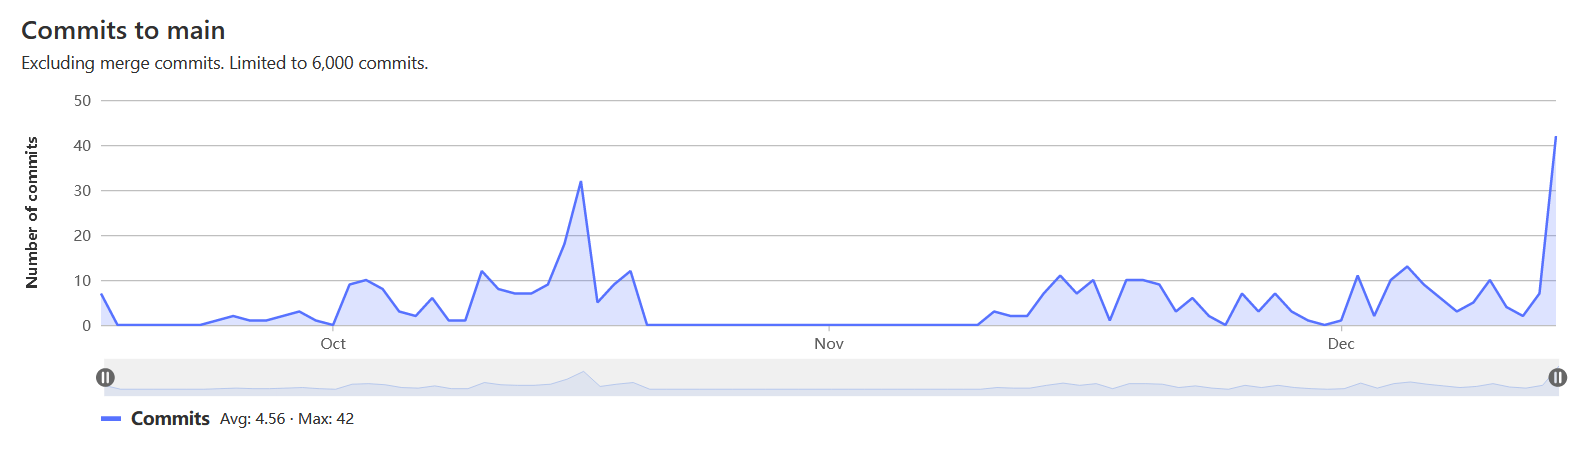
\includegraphics[width= 15 cm, height= 25 cm, keepaspectratio]{slike/CommitsToMain.png} 
				\centering
				\caption{Commitovi na grani main}
				\label{fig:commits}
		\end{figure}

		\begin{figure}[H]
			\begin{minipage}[t]{0.5\textwidth}
				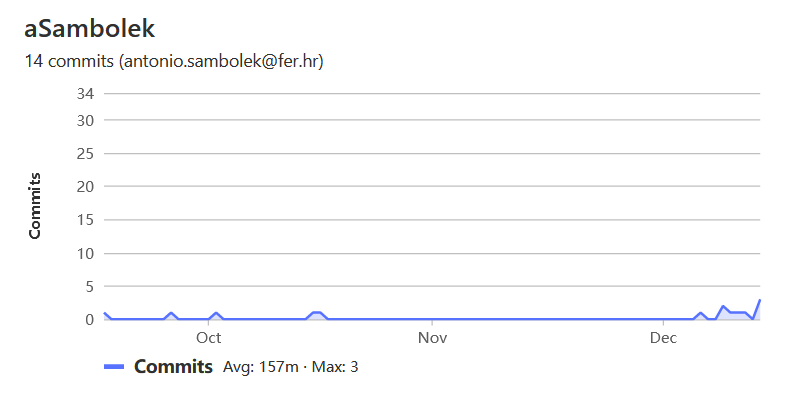
\includegraphics[width=\linewidth]{slike/ASambolek.png}
				\caption{Antonio Sambolek} \label{fig:ASambolek}
			\end{minipage}
			\hspace*{\fill}
			\begin{minipage}[t]{0.5\textwidth}
				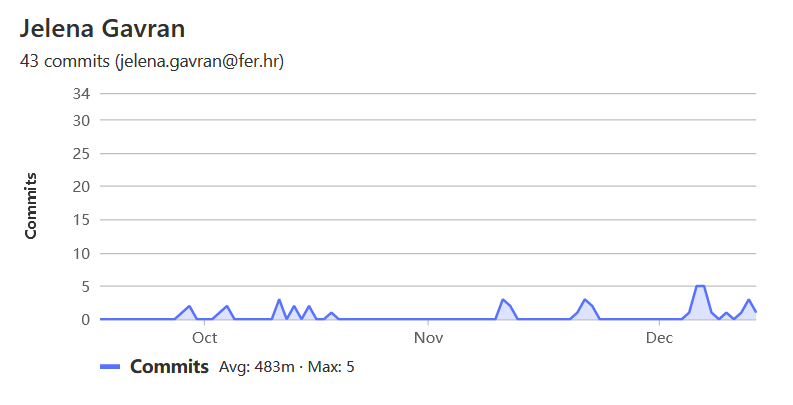
\includegraphics[width=\linewidth]{slike/JGavran.png}
				\caption{Jelena Gavran} \label{fig:Jgavran}
			\end{minipage}
		\end{figure}
		
		\begin{figure}[H]
			\begin{minipage}[t]{0.5\textwidth}
				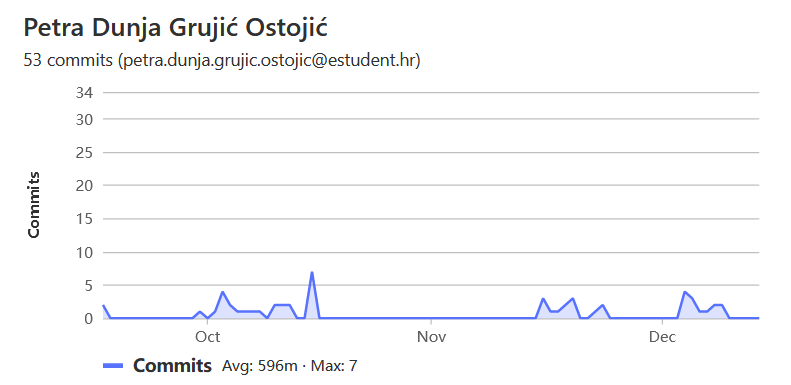
\includegraphics[width=\linewidth]{slike/Petra.png}
				\caption{Petra Dunja Grujić-Ostojić} \label{fig:Petra}
			\end{minipage}
			\hspace*{\fill}
			\begin{minipage}[t]{0.5\textwidth}
				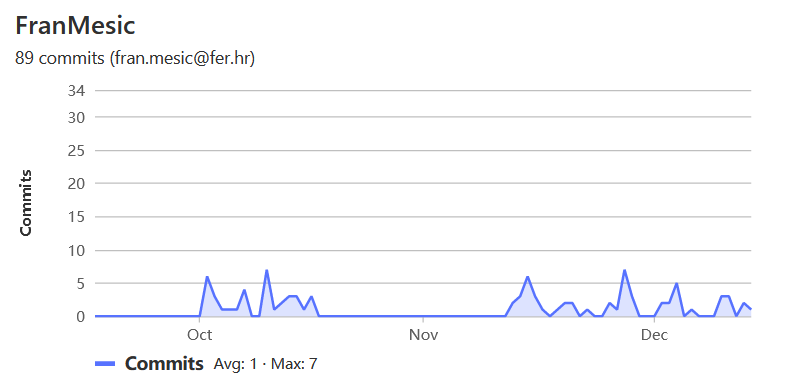
\includegraphics[width=\linewidth]{slike/FMesic.png}
				\caption{Fran Mesić} \label{fig:Fmesic}
			\end{minipage}
		\end{figure}
		
		
		\begin{figure}[H]
			\begin{minipage}[t]{0.5\textwidth}
				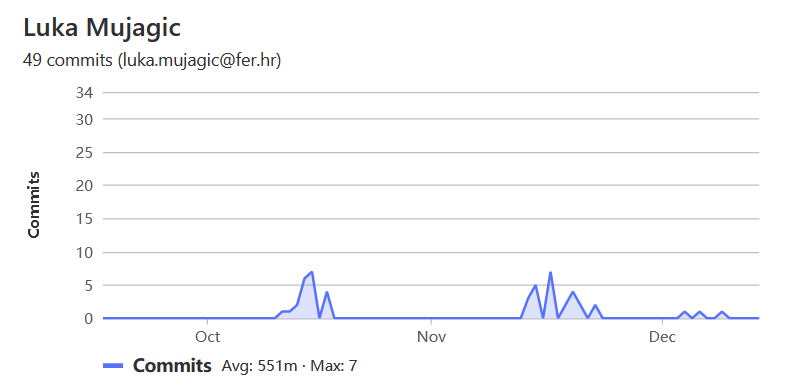
\includegraphics[width=\linewidth]{slike/LMujagic.png}
				\caption{Luka Mujagić} \label{fig:Lmujagic}
			\end{minipage}
			\hspace*{\fill}
			\begin{minipage}[t]{0.5\textwidth}
				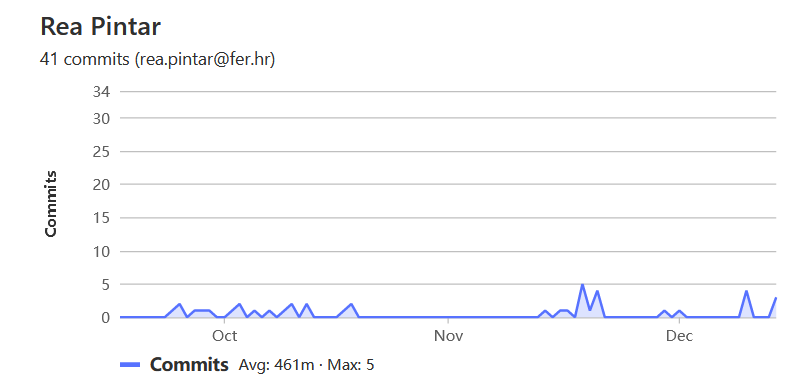
\includegraphics[width=\linewidth]{slike/RPintar.png}
				\caption{Rea Pintar} \label{fig:Rpintar}
			\end{minipage}
		\end{figure}

		\begin{figure}[H]
				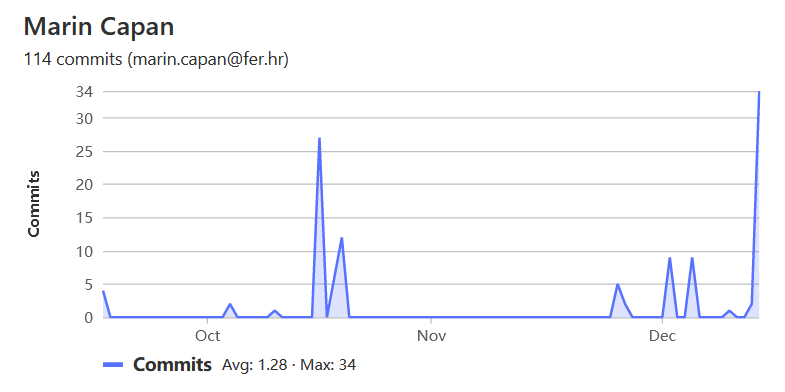
\includegraphics[width= 15 cm, height= 25 cm, keepaspectratio]{slike/MCapan.png} 
				\centering
				\caption{Marin Capan}
				\label{fig:MCapan}
		\end{figure}

		
		
	